\documentclass[10pt]{elsarticle}
\usepackage[utf8]{inputenc}
\usepackage{amsmath,amssymb}
\usepackage{natbib}
\usepackage{graphicx}
\usepackage{caption}
\usepackage{subcaption}
\usepackage{listings}
\usepackage{color}

\definecolor{orange}{rgb}{1,0.5,0}

\lstset{language=C++,
        basicstyle=\ttfamily\footnotesize,
        keywordstyle=\color{blue}\ttfamily,
        stringstyle=\color{red}\ttfamily,
        commentstyle=\color{orange}\ttfamily,
        morecomment=[l][\color{magenta}]{\#},
        numbers=left,
        numberstyle=\tiny,
        frame=tb,
        columns=fullflexible,
        showstringspaces=false
}

\newcommand{\odeint}{\textsc{odeint}}
\newcommand{\Dt}{\Delta t}
\newcommand{\sgn}{\operatorname{sgn}}

% Title Page
\title{Futurization of ODE integration}
\author[cct]{Mario Mulansky}
\ead{mmulansky@cct.lsu.edu}

\author[fau]{Thomas Heller}

\author[cct]{Hartmut Kaiser}

\address[cct]{Center for Computation and Technology -- Lousiana State University, Baton Rouge, USA}

\address[fau]{Friedrich-Alexander University Erlangen-Nuremberg, Germany}

\begin{document}

\begin{abstract}
We present a new approach to parallelization of numerical routines that eliminates the global barriers that are introduced when using standard parallelization techniques.
We show that our new approach can be readily implemented using the high-level HPX-framework.
Furthermore, extensive performance studies are presented in terms of simulations of a dynamical system using the \odeint-library, confirming the superiority of our new approach in cases of inhomogeneous workloads.
\end{abstract}

\maketitle

\section{Introduction}

The recent development in High-Performance Computing (HPC) shows a clear tendency towards heterogeneous multi-core architecture with a prospective availability of exaflop machines with hundreds of millions of cores by the end of this decade.
%~\cite{?}.
This puts out severe challenges for programmers and library authors in how to efficiently utilize the computational power of such machines by suitable parallelization.
In this work, we apply a new parallelization technique to the numerical problem of integration of ordinary differential equations (ODEs).
Solving initial value problems (IVP) of ODEs is an every-day task for scientists and engineers in all subjects.
Hence providing efficient, parallel code for this task is of fundamental importance  with a wide variety of applications.

Here, we will use a new approach to parallelization, called \emph{futurization}~\cite{Heller_Kaiser_Mulansky_tbp}, which will allow us to eliminate the global barriers in the parallelized code and thus reach a better efficiency of the numerical simulations.
The parallelization part of our implementation is based on the HPX library, an experimental implementation of the ParalleX execution model~\cite{Kaiser_Brodowicz_Sterling_09}.
For the numerical algorithm to integrate an ODE we rely on the \odeint\ library, a highly flexible, modern C++ library for solving ODEs~\cite{Ahnert_Mulansky_11}.
We will compare the performance our new approach with a straight-forward OpenMP version of the same algorithm on different dual-processor multi-core machines.

The article is organized as follows.
In the next section we shortly introduce the employed libraries HPX and \odeint, as well as the futurization technique.
Then we outline the parallelization of the numerical simulation in section~\ref{sec:num_ode_int}, and present the performance comparisons in section~\ref{sec:perf}.
Finally, we end with our concluding remarks.

\subsection{HPX}

\subsection{odeint}

The \odeint\ library is a modern C++ implementation of most of the standard algorithms for numerically solving Ordinary Differential Equations (ODEs)~\cite{Ahnert_Mulansky_11} and recently became part of the Boost library collection~\cite{boost}.
It is designed in a highly flexible way, which makes it especially useful for the purpose of this paper.
The fundamental design concept in \odeint\ is the \emph{separation of algorithm and computation}.
This is realized by using modern C++ techniques such as Generic and Template Metaprogramming~\cite{TemplateMetaprogramming}, hence it provides \emph{compile time flexibility} which ensures optimal run-time performance.
This flexibility make \odeint\ applicable for a wide range of problems, for example for performing numerical ODE integration with arbitrary precision, which can be realized simply by combining \odeint\ with an arbitrary precision library like MPFR~\cite{mpfr} or Boost.Multiprecision~\cite{boost_multiprecision}.
Furthermore, it is also possible to introduce parallelization into \odeint\ by simply implementing parallelized computational backends, without needing to re-implement the actual numerical algorithm.
This is a clear advantage when comparing different parallelization techniques like in this article, because it ensures that the numerical schemes are implemented in exactly the same way and any performance difference is solely induced by the different parallelizations.
Hence, \odeint\ is the perfect framework for the purpose of this work.

\subsection{Futurization}

\section{Numerical ODE Integration} \label{sec:num_ode_int}

\subsection{Runge-Kutta Algorithms}

In the following we will show how typical numerical algorithms for finding approximate solutions of such IVP can be parallelized using a dataflow approach.
An IVP of an ODE is defined as:
\begin{equation}
 \dot{\vec x}(t) = \vec f(\vec x(t), t), \qquad \vec x(t=0) = \vec x_0,
\end{equation}
where $\vec x(t) \in \mathbb{R}^N$ is the trajectory in the $N$-dimensional phase space.
To find a numerical solution of this problem, one introduces a time discretization with some step size $\Dt$.
So the numerical solution consists of a sequence of $N$-dimensional points $\vec x_0$, $\vec x_1$, $\vec x_2,\dots$, with $\vec x_n \approx x(n\cdot \Dt)$.
The most important class of schemes are the Runge-Kutta methods, which are explicit one-step methods that use only the previous point $x_n$ to compute the next iterate $x_{n+1}$.
The generic explicit Runge-Kutta scheme with $s$ stages writes as:
\begin{equation} \label{eqn:rk}
 \begin{aligned}
    \vec x_{n+1} &= \vec x_n + \Dt \sum_{k=1}^{s} b_k \vec y_k \\
    \text{where}\quad \vec y_k &= f( \vec x_n + \Dt \sum_{m=1}^k a_{k,m} \vec y_m , t_n+c_k\Dt).
   \end{aligned}
\end{equation}
The parameter sets $a_{k,m}$, $b_k$ and $c_k$ have to be chosen such that the result $x_{n+1}$ is indeed an approximation of some order $p$.
We note that for simplicity we here restrict the study to methods with constant step-size~$\Dt$, but the method below can also be applied to embedded Runge-Kutta schemes required for step size control.
To obtain an approximation of a whole trajectory from $t=0\dots t_\text{end}$ one applies the above one-step algorithm subsequently to obtain a descretized approximate trajectory $\vec x_0,\vec x_1,\vec x_2,\dots,\vec x_T$ with $T=t_\text{end}/\Dt$.

Looking at~\eqref{eqn:rk} one see that the computation of a numerical trajectory consists of two tasks: (i) evaluating the rhs of the ODE $\vec f(\vec x,t)$ and (ii) computing the sum of vector-scalar products $\sum b_k \vec y_k$.
This is also true for more sophisticated numerical scheme like controlled Runge-Kutta schemes, multi-step methods or symplectic routines.
Thus, the parallelization technique described below is not only applicable for the basic Runge-Kutta algorithms~\eqref{eqn:rk}, but can rather be applied to a much broader class of numerical integration schemes.

To parallelize these computations one divides the $N$-dimensional vector $\vec x$ into $M$ sub regions $\vec x^{m}\in \mathbb{R}^{N/M}$ with $m=0\dots M-1$ or $\vec y^{m}$ respectively, which are then distributed across cores/processors/machines and are processed in parallel.
For the vector addition the computations of the sub regions $\vec y^m$ are completely independent from each other, but for the rhs $\vec f(\vec x , t)$ this not the case.
The dependency between the regions is given by the specific problem one is confronted with.
For example, for a system with all-to-all coupling (e.g.\ $N$-body gravitation system), the calculation of one part $\vec y^m$ requires the full state $\vec x^{0}\dots \vec x^{M-1}$.
For the trivial case of an uncoupled system the calculation of $\vec y^m$ only requires the single component $\vec x^m$.
Many systems, however, are somewhere in between these two extreme cases.
Imagine, for example, a problem with nearest neighbor coupling, a very common case in lattice dynamics simulations, then the computation of $\vec y^m$ requires the neighboring components as well: $\vec x^{m-1}$, $\vec x^{m}$ and $\vec x^{m+1}$.
With conventional methods, like OpenMP or MPI, it is not possible, or at least highly cumbersome, to incorporate the dependencies into the parallelized code.
Therefore, a global synchronization is enforced after every rhs evaluation and vector addition step, as shown in Figure~\ref{fig:glob_sync}.

\subsection{Futurized Implementation}

Here we present a new way of parallelizing the algorithm based on dataflow semantics, that will automatically ensure the correct dependencies between the sub-regions of $\vec x^m$.
A natural way of representing the sub-regions $\vec x^m$ in a C++ program is a vector of vectors \lstinline+vector< vector< double > > x+, where \lstinline+x[m]+ represents the $N/M$ dimensional sub-regions $\vec x^m$.
For the futurization of the algorithm one first wraps the plain data into \lstinline+future+ objects holding the data.
Thus, the representation of the regions becomes \lstinline+vector< future< vector< double > > >+, where the future object gets ready as soon as the computation of its data is finished.
Having defined this data structure, it is now very simple to implement a vector-vector addition ready for parallel execution.
Our implementation is based on the \lstinline+hpx::lcos::local::dataflow+ function, that asynchronously applies a functor to a number of future objects.
Exemplarily, we show the code that computes the sum of two vectors $\vec z = \alpha_1 \vec x_1 + \alpha_2 \vec x_2$ in Listing~\ref{lst:hpx_vectoradd}.
There, the calculation for each sub region is assigned to individual tasks and thus can be distributed on the available cores by the HPX scheduler.
\begin{lstlisting}[label=lst:hpx_vectoradd,caption=Futurized vector operation,float=t]
typedef vector< double > sub_state;
typedef vector< future< sub_state > > state;

struct scale_sum2
{
  const double a1 , a2;
  vadd3( double alpha1 , double alpha2 )
    : a1( alpha1 ) , a2( alpha2 ) { }
    
  state operator()( sub_state x1 , sub_state x2 , sub_state x3 )
  {
    for( size_t n=0 ; n<x1.size() ; n++ )
    {
      x1[n] = a1*x2[n]+a2*x3[n];
    }
    return x1;
  }
};

template< typename Operation >
void vector_apply2( state x1 , state x2 , state x3 , Operation op )
{
  for( size_t m=0 ; m<x1.size() ; m++ )
  {
    x1[m] = dataflow( hpx::launch::async , op , x1[m] , x2[m] , x3[m] );
  }
}
...
//calculate z = 0.5*x1 + 0.25*x2
vector_apply( z , x1 , x2 , scale_sum( 0.5 , 0.25 ) );
\end{lstlisting}
The \lstinline+dataflow+ function schedules the execution of the vector operation on the sub-region as soon as all required data is available from the previous operation.
It should be noted that dividing the state into sub-regions in terms of a \lstinline+vector< vector< double > >+ at first looks like a non-continuous memory usage that should lead to a decreased performance.
However, remember that each of the sub-regions will be processed in a separate task, so each core sees continuous data for its computation and the data structure does not influence the performance of the parallelized code.

Secondly, one has to implement the rhs of the ODE.
Here, we will chose an autonomous system with nearest neighbor couplings as an example, but the generalization to other dependencies is rather straight forward.
The rhs of an ODE with nearest neighbor coupling in the most general form writes as:
\begin{equation}
 \dot{\vec x} = \vec f(\vec x):\, x_n = g_n(q_n) + c_{n,l}(q_{n},q_{n-1}) + c_{n,r}(q_{n},q_{n+1}).
\end{equation} 
The function $g_n$ defines the local term at site $n$, while the functions $c_{n,l/r}$ represent the couplings to the left and right.
For simplicity, we will assume that the rhs functions are identical for all lattice sites, and also the left and right coupling is identical, hence: $g_n \equiv g$ and $c_{n,l} \equiv c_{n,r} \equiv c$.
Also, we will employ Diriclet boundary conditions employing that $x[-1] = x[N] = 0$.
The futurized algorithm to compute this function is shown in Listing~\ref{lst:hpx_rhs}.
\begin{lstlisting}[label=lst:hpx_rhs,caption=Futurized rhs function ,float=t]
struct rhs_operation
{
  sub_state operator()( sub_state dxdt , sub_state x , double x_l , double x_r )
  {
    const size_t N = x.size();
    dxdt[0] = g_func( x[0] ) + c_func( x[0] , x_l ) 
			     + c_func( x[0] , x[1] );
    for( size_t n=1 ; n<N-1 ; ++n )
    {
      dxdt[n] = g_func( x[n] ) + c_func( x[n] , x[n-1] ) 
			       + c_func( x[n] , x[n+1] );
    }
    dxdt[N-1] = g_func( x[N-1] ) + c_func( x[N-1] , x[N-2] ) 
				 + c_func( x[N-1] , x_r );
    return dxdt;
  }
};

void rhs( state x , state dxdt , double t )
{
  const size_t M = x.size();
  // boundary condition on the left
  dxdt[0] = dataflow( rhs_operation() , x[0] , dxdt[0] , 
      make_ready_future( 0.0 ) ,
      dataflow( []( sub_state x ){ return x[0]; } , x[1] ) );
  for( size_t m=1 ; m<x.size()-1 ; x++ )
  {
    dxdt[m] = dataflow( rhs_operation() , x[m] , dxdt[m] , 
      dataflow( []( sub_state x ){ return x[x.size()-1]; } , x[m-1] ),
      dataflow( []( sub_state x ){ return x[0]; } , x[m+1] ) );
  }
  // boundary condition on the right
  dxdt[M-1] = dataflow( rhs_operation() , x[M-1] , dxdt[M-1] , 
      dataflow( []( sub_state x ){ return x[x.size()-1]; } , x[M-2] ),
      make_ready_future( 0.0 ) );
}
\end{lstlisting}
Note, how in the function \lstinline+rhs+ dataflows are used to extract the first/last value of the neighboring regions and pass them into the next dataflow (e.g.\ Lines 29,30 in Listing~\ref{lst:hpx_rhs}).
That implies that the dataflow for calculating the rhs for the $m$-th sub-region gets input from the regions $m-1$, $m$ and $m+1$.
This is exactly the constitution of the dependencies of the nearest neighbor coupling.
With this technique, the computation of the rhs function for region $m$ starts as soon as all the required data is available, even if some other sub-regions are not yet computed.

\begin{figure}
 \begin{subfigure}[b]{0.49\textwidth}
  \centering
  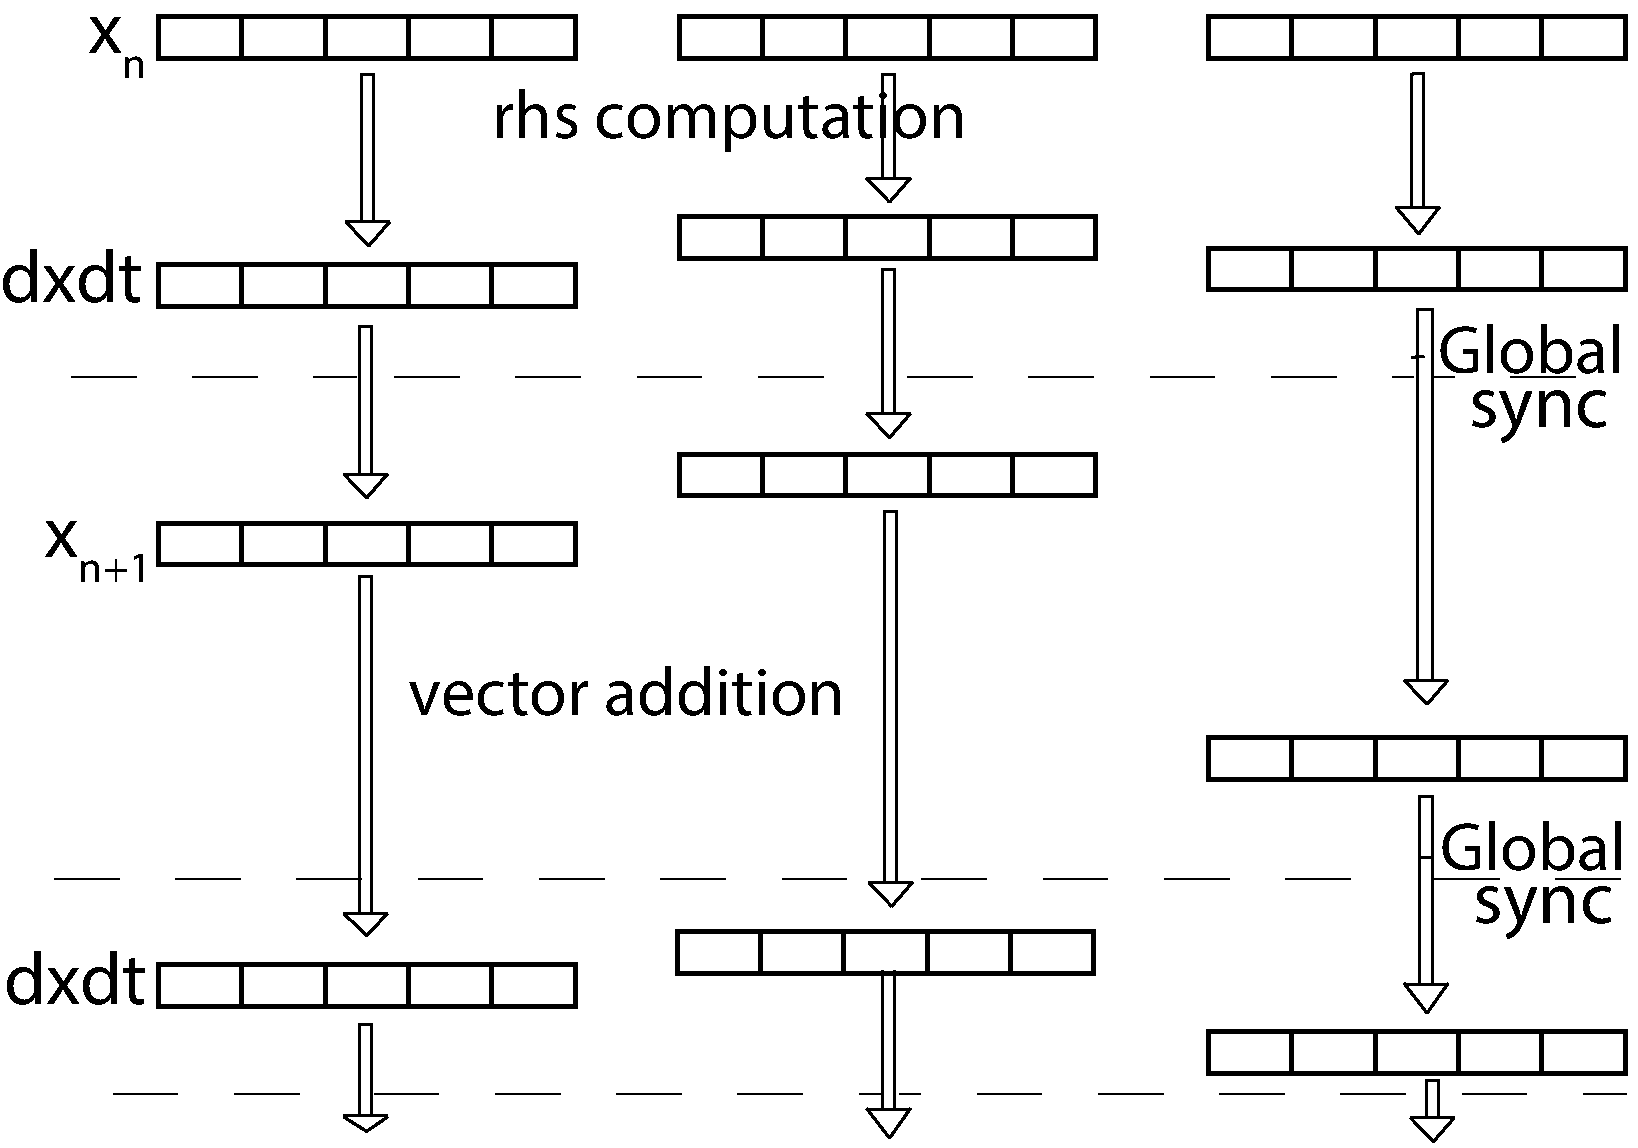
\includegraphics[width=0.95\textwidth]{par_global.pdf}
  %{parallelization_global.png}
  \caption{Parallelization with global barriers.}
  \label{fig:par_glob_bar}
 \end{subfigure}\vline
 \begin{subfigure}[b]{0.49\textwidth}
  \centering
  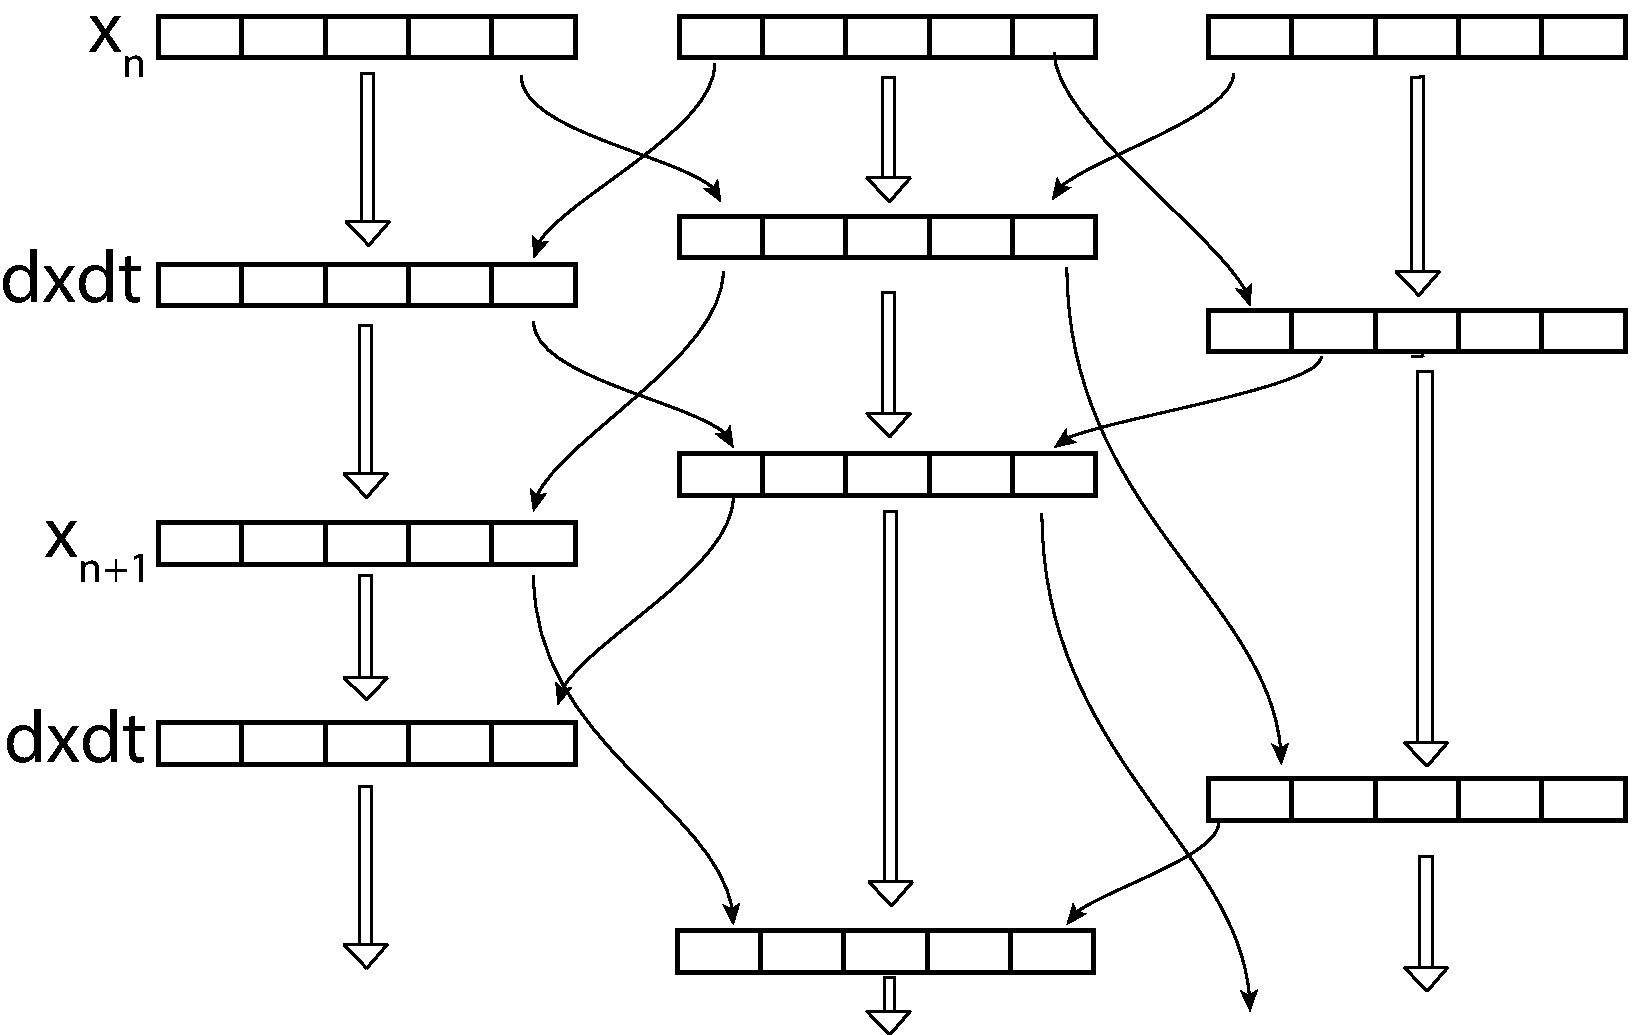
\includegraphics[width=0.95\textwidth]{par_dfo.pdf}\vspace{1em}
  \caption{Parallelization by futurization.}
  \label{fig:par_fut}
 \end{subfigure}
 \caption{Comparison of the execution flow using OpenMP parallelization which introduces global barriers (a) and the new futurization technique that accounts for the actual data dependencies (b).} 
 \label{fig:parallelization}
\end{figure}

In contrast, an OpenMP implementation of the rhs function is exemplarily shown in Listing~\ref{lst:omp_rhs}.
\begin{lstlisting}[label=lst:omp_rhs,caption=OpenMP rhs function,float=t]
void rhs( state x , state dxdt , double t )
{
  const size_t M = x.size();
  const size_t L = x[0].size();
  rhs_operation op;
#pragma omp parallel for schedule(static)
  for( size_t m=0 ; m<M ; ++m )
  {
    if( m==0 )
      dxdt[0] = op( x[0] , 0.0 , dxdt[1][0] );
    elseif( m<M-1 )
      dxdt[m] = op( x[m] , dxdt[m-1][L-1] , dxdt[m+1][0] );
    else
      dxdt[M-1] = op( x[M-1] , dxdt[M-2][L-1] , 0.0 );
  }
}
\end{lstlisting}
Note that here, the parallel code is only entered when the full state $\vec x$ is calculated completely.
Additionally, at the end of the parallel OpenMP region a global synchronization takes place.
The difference in the execution flow of these two methods is visualized in Figure~\ref{??}.
We also want to emphasize that the HPX and the OpenMP implementation work with the same kernel functor \lstinline+rhs_operation+, defined in the beginning of Listing~\ref{lst:hpx_rhs}.
This represents an important aspect of futurization, namely that the fundamental numerical computations remain the same, but only get wrapped into future objects that define the data dependencies.

It is clear that for the case of identical computation for all sub-regions ($g_n$ and $c_n$ independent of $n$) and in a homogeneous multi-core environment, the punishment of a global synchronization at each step is not expected to be of significant impact.
However, we still compare the new futurization approach based on HPX with a standard OpenMP implementation for exactly such a case and we will find that the HPX code is competitive even in this setting highly favorable for OpenMP, as described next.
Furthermore, changing the workload to an inhomogeneous setup, where each core gets different amounts of computation, should change this picture in favor of HPX with absent global barriers.
This will also be addressed in the next part.

\section{Performance} \label{sec:perf}

\subsection{Homogeneous Work Distribution}

As example system for our performance comparison we choose a Hamiltonian system of nonlinearly coupled anharmonic oscillators.
The equations of motions for a one-dimensional chain of such oscillators is:
\begin{equation}
 \dot p_n = -|q_n|^\kappa\sgn(q_n) - |q_n-q_{n-1}|^\lambda\sgn(q_n-q_{n-1}) - |q_n-q_{n+1}|^\lambda\sgn(q_n-q_{n+1}).
\end{equation} 
Hence, the functions from above are given as $g(x) = |x|^\kappa\sgn(x)$ and $c(x,y)=|x-y|^\lambda\sgn(x-y)$, where $\sgn(x)$ is sign of $x$.
This model with integer powers $\kappa$ and $\lambda$ has been studied extensively by theoretical physicists in the context of Hamiltonian Chaos~\cite{Mulansky-Ahnert-Pikovsky-Shepelyansky-11} and Chaotic Diffusion~\cite{Mulansky_Pikovksy_12,mulansky2013energy,Mulansky_phd_12}.
Here, we will use (arbitrary) non-integer powers $\kappa=2.3$ and $\lambda=3.7$, which makes the system even more computationally demanding.
As the numerical integrator we use a fourth order symplectic Runge-Kutta scheme~\cite{McLachlan_95}.
The symplectic nature of this scheme preserves the Hamiltonian character of the system and is thus more suitable than a generic Runge-Kutta algorithm.
However, from a computational point of view this scheme requires the same kind of numerical calulcations (rhs evaluation, vector additions) as described above.

\begin{figure}
 \begin{subfigure}[b]{0.49\textwidth}
  \centering
  \includegraphics[width=\textwidth]{ariel_granularity.pdf}
  \caption{Influence of granularity.}
  \label{fig:granularity_ariel_1024K}
 \end{subfigure}
 \begin{subfigure}[b]{0.49\textwidth}
  \centering
  \includegraphics[width=\textwidth]{ariel_flops.pdf}
  \caption{FLOP/Cycle on many cores.}
 \end{subfigure}
 \caption{(a) Runtime of 100 steps of a system of size $N=1048576$ with 16 Threads for different granularities (data per task) using the Intel Compiler. (b) Performance in FLOP per CPU cycle per Core for the g++ and Intel Compiler.} 
 \label{fig:ariel_flops}
\end{figure}

To compare the performance of the dataflow driven algorithm based on HPX with a straight forward OpenMP implementation we ran simulations for the model described above with $N$ lattice sites.
%and $N=512\cdot1024$ and $N=1024\cdot1024$.
Our main test system is dual processor machine with two Xeon E5-2690 Sandy Bridge processors.
For compilation we use the GNU compiler 4.7.3 as well as the Intel compiler 13.0.1.
As explained above, for each computation the chain is divided into chunks of size $G=N/M$ and distributed across the cores, hence each core is assigned the same workload.
First, we checked the influence of the chunk size $G$ on the performance.
In Figure~\ref{fig:granularity_ariel_1024K} we show the runtime of 100 time steps of the simulation for a chain of $N=1024\cdot1024$ oscillators, using the Intel compiler.
For the HPX code one clearly sees a minimum for a data amount of 32K/task, while the OpenMP code shows almost no dependence on the granularity.
Therefore, one should always test for the optimal granularity setting when using HPX.
Moreover, the results in Figure~\ref{fig:granularity_ariel_1024K} suggest that the OpenMP version is about 10\% faster than HPX.
We verified this in a second study where we measured the floating point operations per second (FLOP/s) with help of the \lstinline+likwid+ tool~\cite{likwid}.
We normalized this performance number to the clock speed of the processor and obtained the numbers of floating point operations per cycle (FLOP/cycle).
This is necessary to make runs on different numbers of cores comparable, because the Xeon machine increases the CPU clock speed if only a few cores are utilized.
The results are shown in Figure~\ref{fig:ariel_flops}.
One first notes that for the GNU compiler the performance of OpenMP and HPX is identical with a perfect scaling up to 16 cores.
However, the Intel compiler gives almost twice the performance as the GNU compiler, and there we indeed see that the OpenMP code is about 10\% faster than HPX.
But again, the performance of each core remains constant when going from one to 16 cores for both the OpenMP and the HPX implementation.
Hence we found that both the HPX and the OpenMP code for both the GNU and the Intel Compiler exhibits perfect scaling.
However, from here on we will focus on the performance obtained using the Intel Compiler, as it generates gives significantly faster code.

\begin{figure}
 \begin{subfigure}[b]{0.49\textwidth}
  \centering
  \includegraphics[width=\textwidth]{ariel_scaling_1024K.pdf}\hfill
  \caption{Performance with 1024K lattice sites.} 
  \label{fig:scaling_ariel_1024K}
 \end{subfigure}
 \begin{subfigure}[b]{0.49\textwidth}
  \centering
  \includegraphics[width=\textwidth]{marvin_scaling_512K.pdf}\hfill
  \caption{Performance with 512K lattice sites.} 
  \label{fig:scaling_marvin_512K}
 \end{subfigure}
 \caption{Strong scaling for a system of size $N=1048576$ on a 2xXeonE5-2690 (a) and $N=524288$ on a 2xXeonE5-2450 (b). The diamonds (``HPX gb'') represents the performance of a simulation using HPX with additional global barriers. All curves are normalized to the single core performance.
 }
 \label{fig:scaling1D}
\end{figure}

This is again visualized in Figure~\ref{fig:scaling1D}.
There, we show the efficiency of the parallelization defined as $\text{Eff} = \tau_1/(\tau_C\cdot C) \cdot100\%$, where $\tau_1$ is the run time of the simulation on a single core, and $\tau_C$ is the run time on $C$ cores.
Hence, all the graphs in Figure~\ref{fig:scaling1D} are normalized to a single thread run.
Figure~\ref{fig:scaling_ariel_1024K} shows the results for N=$1024\cdot1024$ oscillators on the XeonE5-2690 machine, while in \ref{fig:scaling_marvin_512K} we used N=$512\cdot1024$ oscillators and performed the simulations on a slower 2xXeonE5-2450 blade.
Both implementations exhibit almost perfect scaling up to the 16 cores of the dual eight-core processor machines.
On both machines, the OpenMP code with the Intel compiler and static scheduling gives the fastest results, hence we used these runs as reference defining 100\%.
One finds that the HPX implementation is about 10\% slower than static OpenMP scheduling, but overtakes the dynamic OpenMP runs when going using all 16 cores.
The diamonds represent an HPX implementation where global barriers after each rhs computation were added artificially.
Indeed one finds a severe performance decrease in this case.
Thus, we find indeed that the HPX implementation benefits greatly from the dataflow driven computation, showing the strength of this concept.

\subsection{Inhomogeneous Work Distribution}

The case above represents perfect conditions for OpenMP, as each thread gets assigned the same workload which means that the implicit global barriers of the OpenMP code should not be too important.
A much more interesting case is when the different tasks represent different workloads.
Then, the existence of global barriers might significantly decrease the efficiency of the parallelization when the cores with less work have to wait for the rest.
Such situations can happen frequently in the context of ODE integration, for example when the ODE is obtained from an underlying partial differential equation using an adaptive grid, a situation one face rather typically in hydrodynamic simulations.
Another example are studies of heterogeneous systems, e.g.\ studying the transport through a chain of nonlinear oscillators enclosed by linear oscillators to the left and right.
Also, a system with some parts being connected to a heat bath, as studied extensively in the context of heat transport~\cite{Lepri_Livi_Politi_03}, gives rise to a heterogeneous system that would create different work loads when parallelizing.

\begin{figure}
 \begin{subfigure}[b]{0.49\textwidth}
  \centering
  \includegraphics[width=\textwidth]{marvin_inhom_granularity.pdf}\hfill
  \caption{Granularity, inhomogeneous workload.} 
  \label{fig:inhom_granularity}
 \end{subfigure}
 \begin{subfigure}[b]{0.49\textwidth}
  \centering
  \includegraphics[width=\textwidth]{marvin_scaling_inhom_512K.pdf}\hfill
  \caption{Efficiency, inhomogeneous workload.} 
  \label{fig:inhom_512K}
 \end{subfigure}
 \caption{Influence of the average granularity on the performance (a) and efficiency of the parallelization (b) for the case of inhomogeneous workloads using the Intel compiler on the 2xXeonE5-2450 machine for a chain of size $N=524288$. The granularity was measured using all 16 Cores, with dynamic scheduling for OpenMP.}
 \label{fig:inhom_1}
\end{figure}

\begin{figure}
 \begin{subfigure}[b]{0.49\textwidth}
  \centering
  \includegraphics[width=\textwidth]{comp_hom_inhom_marvin.pdf}
  \caption{Comparison of workload distributions.} 
  \label{fig:comp_hom_inhom_marvin}
 \end{subfigure}
 \begin{subfigure}[b]{0.51\textwidth}
  \centering
  \includegraphics[width=0.95\textwidth]{scaling_inhom_1024K_128K.pdf}
  \caption{Different problem sizes.} 
  \label{fig:inhom_1024K}
 \end{subfigure}
 \caption{Panel (a) shows a comparison of the homogeneous and inhomogeneous workload distribution for OpenMP with dynamic scheduling and HPX on 16 Cores of the XeonE5-2450 machine. We plot the performance in terms of simulation steps per second for a system size $N=524288$. Panel (b) shows the parallel efficiency for a system of size $N=1048576$ on the XeonE5-2690 machine, and $N=131072$ on the XeonE5-2450.}
 \label{fig:inhom_2}
\end{figure}

Here, we mimic such a situation by dividing the vector $\vec x$ into subregion of different sizes.
Then, instead of having the same workload for each task, now the amount of data to be processed differs.
Specifically, we divide the state into $M$ subregions of length $G_m$, where $G_{2k}=G/2$ and $G_{2k+1}=3G/2$ with $G=N/M$.
Hence, on average every task gets the same workload as above, but now regions with even index have less elements ($G/2$), while those with odd index have more ($3G/2$).

We perform the same study as above for this situation of inhomogeneous workload distribution.
The results are shown in Figure~\ref{fig:inhom_1}.
As expected, OpenMP with static scheduling now shows much worse performance, seen in Figure~\ref{fig:inhom_512K}, because the program can not adjust to the fact that some threads finish earlier than others.
We also notice that the OpenMP code becomes much more sensitive to the granularity, as shown in Figure~\ref{fig:inhom_granularity}, where we show the run time of the simulation on all 16 cores of the  2xXeonE5-2450 machine for a chain of size $N=524288$ and dynamic scheduling for OpenMP.
Additionally, we already see there that the HPX implementation shows a about 15\% better performance on 16 cores.
To verify this we again measure the efficiency of the parallelization normalized to the single-core run, as explained above.
The result is shown in Figure~\ref{fig:inhom_512K}.
When running on less than eight cores, the OpenMP code is still slightly faster, but for 16 cores HPX takes over and wins by about 10\%.
This is very similar to the observation with homogeneous workloads, where also HPX was faster than OpenMP with dynamic scheduling, cf.\ Figure~\ref{fig:scaling_marvin_512K}.
However, now the static scheduling is not an option and thus HPX provides the overall fastest solution, at least for large numbers of cores.

It is very interesting to note that the HPX implementation is equally efficient for homogeneous and inhomogeneous workload distributions.
This is emphasized in Figure~\ref{fig:comp_hom_inhom_marvin}, where we plot the performance in terms of simulation steps per seconds for homogeneous and inhomogeneous workload distributions.
While the two graphs for HPX lie exactly on top of each other, the OpenMP performance drops slightly for the inhomogeneous version.
Hence, the dataflow driven implementation with HPX allows to use the available computational power maximally efficiently also in cases of inhomogeneous workloads.
Figure~\ref{fig:inhom_1024K} shows the efficiency of the parallelization for an inhomogeneous workload for a larger system with $N=1048576$ on the 2xXeonE5-2690 machine and a smaller system with $N=131072$ on the 2xXeonE5-2450.
While for larger systems the OpenMP code becomes more efficient, at smaller system sizes, i.e.\ less computational workload, the advantage of HPX becomes more pronounces.
Hence, we find that HPX very well suited for inhomogeneous situations even outperforming Intel's OpenMP implementation when running on 16 Cores.
This is not surprising, because it is exactly when the dataflow driven parallelization with the absence of global barriers is superior, nicely verified in these simulations.

\subsection{2D Simulations}

One-dimensional systems with $10^6$ sites, as simulated above, are indeed important, for example when exploring the thermodynamic limit.
However, a more common application for parallelization are studies of higher dimensional systems.
Hence, we also implemented an OpenMP and HPX version of a 2D lattice simulation of the above model.
Note, that in two dimensions one has additional coupling terms.
Here, we chose a quadratic lattice where each oscillator is coupled to its four nearest neighbors.
Although the rhs function gets more cumbersome to implement, the algorithm is conceptually the same and it is rather straight forward, how the above code is generalized to a 2D simulation.
The only detail that should be mentioned is that we divided the 2D lattice into rectangular stripes of some width $G$ and length $N$ and distributed those stripes across the available cores.
One could also divide the lattice into quadratic regions, but this is not expected to have a significant influence on the performance.

\begin{figure}
 \begin{subfigure}[b]{0.49\textwidth}
  \centering
  \includegraphics[width=\textwidth]{ariel_strong_scaling.pdf}\hfill
  \caption{Strong scaling of the 2D simulation.} 
  \label{fig:strong_scaling2D}
 \end{subfigure}
 \begin{subfigure}[b]{0.49\textwidth}
  \centering
  \includegraphics[width=\textwidth]{ariel_weak_scaling.pdf}\hfill
  \caption{Weak scaling of the 2D simulation.} 
  \label{fig:weak_scaling2D}
 \end{subfigure}
 \caption{Strong (a) and weak (b) scaling for the 2D simulation on the 2xXeonE5-2690 machine using the Intel compiler. In both graphs the results are scaled to the OpenMP single thread performance. For the weak scaling results the data size per thread was fixed to $512\times512$.}
 \label{fig:marvin_scaling2D}
\end{figure}

Again, we compare the run-time of the OpenMP and HPX parallelization.
In Figure~\ref{fig:strong_scaling2D} we show the strong scaling results on the Intel XeonE5-2690 machine using the Intel compiler.
As above, we used the OpenMP single-core performance to represent 100\% in these graphs.
Like before, we find very good scaling of the parallel codes, with a slightly better performance of the OpenMP implementation for most cases.
However, for the largest case of $N=2048\times2048$ on 16 Cores, the HPX code is slightly faster.
Figure~\ref{fig:weak_scaling2D} shows the weak scaling of these simulation, again exhibiting almost perfect scaling with about 90\% of the theoretical optimum at 16 threads and a slightly better performance of HPX over OpenMP on 16 threads.


\section{Conclusions} \label{sec:conc}

We presented a new technique to parallelize ODE solvers based on the HPX and odeint libraries, namely by futurization.
Our implementation is based on a dataflow driven scheduling as provided by HPX.
This allows the programmer to specifically define data dependencies, which in the case of ODE integration are manifestations of the coupling terms.
Having those data dependencies, the scheduler can efficiently distribute the computation as soon as all required data is available.
Using the highly flexible odeint library, the futurization technique can be implemented quite easily by providing suitable computation backends without requiring to re-implement the actual numerical algorithms.

We executed several performance test comparing our new approach with standard OpenMP parallelization.
For a homogeneous workload, we found that in all cases our implementation exhibits perfect scaling up to the 16 Cores of our dual processor Intel Xeon machines.
Using the GNU compiler, we found exactly identical performance for our HPX and the OpenMP codes.
The Intel compiler, however, was able to utilize the Xeon processors more efficiently and produced almost two times faster code than the GNU compiler.
Furthermore, we find that the Intel's OpenMP implementation with static scheduling always gives the best performance, being about 10\% faster than HPX.
When using the dynamic scheduling in OpenMP, this changes and we find that the HPX implementation becomes faster than OpenMP when running on 16 cores.
In a heterogeneous situation, where different threads get assigned different workloads, static scheduling is not an option and we find HPX to beat OpenMP by about 10\% in some of our performance tests.
This shows the strength of the dataflow driven, futurized algorithm where the absence of global barriers allows for a more efficient utilization of the available cores.
We also showed some performance results for 2D systems, where HPX is again highly competitive, even exhibiting slight advantages for large systems on 16 cores.
We conclude that a dataflow driven ODE integration based on HPX and odeint is a powerful new approach to parallelization.
Even for cases that favor standard parallelization techniques such as OpenMP, we found competitive performance of our implementation.
Going to more complex cases with inhomogeneous workloads, the HPX based implementation starts outperforming OpenMP when fully utilizing all available cores.

\section*{Acknowledgements}

M.M.\ acknowledges financial support from the German Academic Exchange Foundation (DAAD) and thanks the Center of Computation and Technology for its hospitality.
We thank M.~Camarena for creating the graphs.

\bibliographystyle{unsrt}
\bibliography{articles}

\end{document}
